% inspiration for this figure was drawn from the following animation:
% https://www.youtube.com/watch?v=5A39Ht9Wcu0

\documentclass[border=3pt,tikz]{standalone}
\usepackage{tikz}
\usepackage[outline]{contour} 
\usetikzlibrary{calc}
\usepackage{pgfplots}
\pgfplotsset{compat=1.18}


\begin{document}

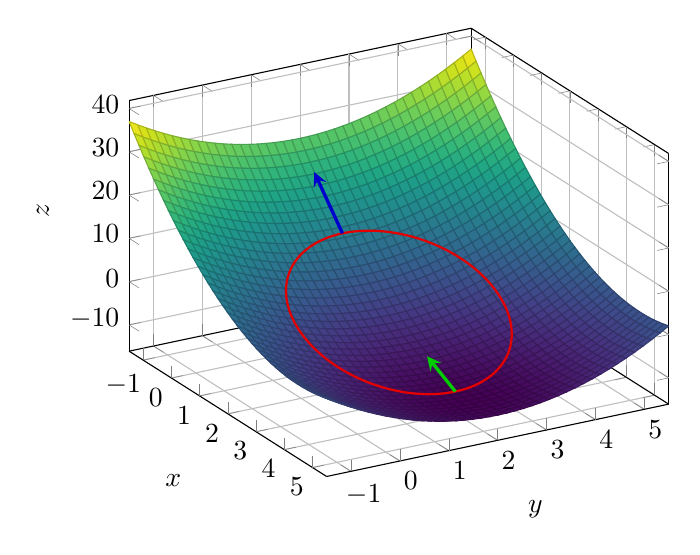
\begin{tikzpicture}
  \begin{axis}[grid,
    view={60}{30},
    domain=-1.5:5.5,
    domain y=-1.5:5.5,
    xtick distance=1,
    ytick distance=1,
    ztick distance=10,
    samples=41,
    xlabel={$x$},
    ylabel={$y$},
    zlabel={$z$},
    colormap/viridis,
    shader=interp
  ]
  
    % Surface: f(x,y) = (x-3)^2 + (y-2)^2 - 3x = z
    \addplot3[
      surf,
      shader=faceted
    ]
    { (x-3)^2 + (y-2)^2 - 3*x };

    % Red curve on the surface: (x-2)^2 + (y-2)^2 = 4 (the constriction)
    % Parametrisation: x = 2 + 2 cos t, y = 2 + 2 sin t
    \addplot3[
      thick,
      red!90!black,
      samples=200,
      domain=0:360,
      samples y=0
    ]
    (
      { 2 + 2*cos(x) },   % x(t)
      { 2 + 2*sin(x) },   % y(t)
      {
        (2 + 2*cos(x) - 3)^2
        + (2 + 2*sin(x) - 2)^2
        - 3*(2 + 2*cos(x))
      }                   
    );

    % gradient vectors in -x direction at (4,2) and (0,2)
    % z values at these points
    \pgfmathsetmacro{\zAb}{(4-3)^2 + (2-2)^2 - 3*4}  % (4,2)
    \pgfmathsetmacro{\zAe}{(4-3)^2 + (3-2)^2 - 3*3}  % (3,2)
    \pgfmathsetmacro{\zBb}{(0-3)^2 + (2-2)^2 - 3*0}  % (0,2)
    \pgfmathsetmacro{\zBe}{((-1)-3)^2 + (2-2)^2 - 3*(-1)}  % (-1,2)

    % Vector at (4,2,f(4,2)) in -x direction
    \addplot3[
      very thick,
      green!80!black,
      -stealth
    ]
    coordinates {
      (4,2,\zAb)
      (3,2,\zAe)
    };

    % Vector at (0,2,f(0,2)) in -x direction
    \addplot3[
      very thick,
      blue!80!black,
      -stealth
    ]
    coordinates {
      (0,2,\zBb)
      (-1,2,\zBe)
    };
  \end{axis}
\end{tikzpicture}




\usetikzlibrary{calc}

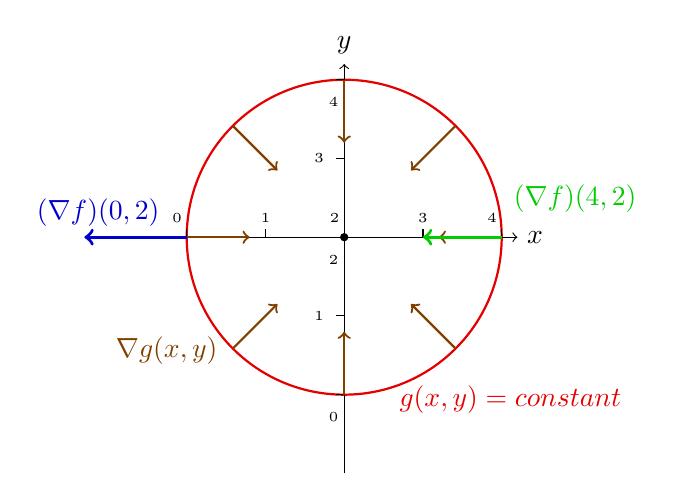
\begin{tikzpicture}[scale=1]
  % Circle: (x-2)^2 + (y-2)^2 = 4 = g(x,y)
  \draw[thick, red!90!black] (2,2) circle[radius=2] node[right=60, below=50] {$g(x,y)=constant$};

  % Axes
  \draw[->] (-1,2) -- (4.2,2) node[right] {$x$};
  \foreach \x in {1,3} \draw (\x,2) -- (\x,2.1) node[above=-1] {\tiny $\x$};
  \foreach \x in {0,2,4} \draw (\x,2) -- (\x,2.1) node[left=3.5,above=-1] {\tiny $\x$};
  \draw[->] (2,-1) -- (2,4.2) node[above] {$y$};
  \foreach \y in {1,3} \draw (2,\y) -- (1.9,\y) node[left=1] {\tiny $\y$};
  \foreach \y in {0,2,4} \draw (2,\y) -- (1.9,\y) node[left=1, below=3] {\tiny $\y$};

  % Inward normal arrows (the gradient of the surface g, defined as g(x,y) = (x-2)^2 + (y-2)^2 )
  \foreach \ang in {0,45,90,135,180,270,315} {
    \coordinate (P) at ({2+2*cos(\ang)},{2+2*sin(\ang)});

    % Inward normal arrow: from P towards centre
    \draw[->,thick,orange!50!black] (P) -- ++({-0.8*cos(\ang)},{-0.8*sin(\ang)}) coordinate (N);
    }
  \foreach \ang in {225} {
    \coordinate (P) at ({2+2*cos(\ang)},{2+2*sin(\ang)});

    % Inward normal arrow: from P towards centre
    \draw[->,thick,orange!50!black] (P) -- ++({-0.8*cos(\ang)},{-0.8*sin(\ang)}) coordinate (N) node[left=40, below=8] {$\nabla g(x,y)$};
    }
    

  % Extra blue vectors in -x direction
  \draw[->,very thick,green!80!black] (4,2) -- ++(-1,0) node[left=-55, above=5] {$(\nabla f)(4,2)$};   % from (4,2)
  \draw[->,very thick,blue!80!black] (0,2) -- ++(-1.3,0) node[left=-5, above] {$(\nabla f)(0,2)$}; % slightly longer from (0,2)

  % Mark the centre
  \fill (2,2) circle[radius=1.5pt];
\end{tikzpicture}



\end{document}